\documentclass[journal,10pt,twocolumn]{IEEEtran}
\usepackage{cite}
\usepackage{amsmath,amssymb,amsfonts}
\usepackage{algorithmic}
\usepackage{graphicx}
\usepackage{textcomp}
\usepackage{xcolor}
\usepackage{booktabs}
\usepackage{array}
\usepackage{url}

\graphicspath{{results/graphs/}}

\begin{document}

\title{GridBalance --- Hybrid Grey Wolf--PSO for\\Renewable Micro-Grid Load Dispatch\\
\large Comprehensive Research and Technical Project Report}

\author{
    \IEEEauthorblockN{Jay Kushwaha}
    \IEEEauthorblockA{\textit{Department of Artificial Intelligence and Machine Learning} \\
    \textit{Lovely Professional University, Phagwara, Punjab} \\
    Email: Jaykushwaha8994@gmail.com}
    \and
    \IEEEauthorblockN{Kriti Nishad}
    \IEEEauthorblockA{\textit{Department of Artificial Intelligence and Machine Learning} \\
    \textit{Lovely Professional University, Phagwara, Punjab} \\
    Email: kritinishad20@gmail.com}
    \and
    \IEEEauthorblockN{\phantom{.} \\ Dr}
    \IEEEauthorblockA{\textit{Department of Artificial Intelligence and Machine Learning} \\
    \textit{Associate Professor in School of Computing and AI} \\
    \textit{Lovely Professional University, Phagwara, Punjab}}
}

\maketitle

\begin{abstract}
Optimal load dispatch in modern renewable microgrids requires coordinated scheduling of intermittent distributed generation (DG) assets, electrochemical energy storage systems, and utility grid interconnections under dynamic time-of-use (TOU) tariffs. This technical report presents the comprehensive mathematical formulation, algorithmic architecture, software implementation, and empirical verification of GridBalance---a research-grade microgrid economic dispatch optimization framework. Authentic solar photovoltaic (PV) and distributed wind power time-series from the Nature Scientific Data DDRE-33 dataset (mapped to the standard IEEE 33-bus radial distribution network) are integrated with a 2.0 MWh Lithium-Iron-Phosphate (LFP) Battery Energy Storage System (BESS). To resolve the non-convex dispatch problem, we benchmark Particle Swarm Optimization (PSO), Grey Wolf Optimizer (GWO), a Genetic Algorithm (GA), and an adaptive Hybrid GWO--PSO engine across 10 random seeds (40 total benchmark runs, $N=30$, $K=100$). The model incorporates a cyclic terminal battery State of Charge (SOC) constraint ($|\text{SOC}(24) - \text{SOC}(0)| \le 1.0\%$) to prevent artificial energy depletion, and an explicit power balance formulation tracking unserved load and excess generation without silent clipping. Results demonstrate that all 40 runs achieve 100.0\% physical feasibility with zero unserved energy and machine-precision power balance ($|\text{residual}| \le 2.27 \times 10^{-13}$ kW). Hybrid GWO--PSO achieves superior stability (standard deviation \$45.09 vs \$82.47 for PSO) and statistically significant cost reduction over standalone GWO (Welch's $t = -3.505$, $p = 0.0031$; Mann-Whitney $U = 9.0$, $p = 0.0022$), providing an average daily operational saving of \$97.68.
\end{abstract}

\begin{IEEEkeywords}
Renewable Microgrid Dispatch, Hybrid Grey Wolf Optimization, Particle Swarm Optimization, Battery Energy Storage Conservation, DDRE-33 Dataset, Power Balance Identity, Metaheuristic Benchmarking, Statistical Significance Testing.
\end{IEEEkeywords}

\section{Introduction and Problem Statement}
\IEEEPARstart{I}{ntegrating} distributed energy resources (DERs)---predominantly solar photovoltaics (PV) and wind energy conversion systems (WECS)---into distribution networks offers substantial carbon abatement and operational cost reductions. However, their intermittent generation introduces steep ramping requirements and power balancing challenges. Battery Energy Storage Systems (BESS) provide temporal buffering, charging during low-tariff or high-renewable intervals and discharging during peak-tariff windows.

Mathematically, the microgrid economic load dispatch problem is a non-linear, constrained optimization task. Conventional mathematical programming techniques (such as mixed-integer linear programming or sequential quadratic programming) often require linearizations that oversimplify non-linear battery degradation mechanisms, non-linear tariff schedules, or complex physical constraints. Metaheuristic algorithms have thus garnered widespread research interest.

Nonetheless, standard Particle Swarm Optimization (PSO) frequently suffers from premature convergence in multi-dimensional dispatch landscapes, becoming trapped in sub-optimal local minima. Conversely, the Grey Wolf Optimizer (GWO) provides superior global exploration through its multi-leader social hierarchy but often exhibits slower convergence in the fine-tuning exploitation phase.

Furthermore, a critical flaw identified across prior microgrid dispatch literature is the omission of cyclic battery state-of-charge (SOC) terminal constraints. An unconstrained optimizer will aggressively deplete initial battery energy (e.g., from 50\% to 20\%), reporting artificially low operational costs by consuming ``free'' stored energy without accounting for terminal replenishment. Similarly, naive clipping of utility grid exchange creates hidden energy imbalances. This report details GridBalance, which resolves these mathematical and algorithmic vulnerabilities.

\section{DDRE-33 Dataset and System Architecture}

\subsection{The DDRE-33 Empirical Dataset}
The project integrates empirical time-series data from the official DDRE-33 benchmark dataset published in Nature Scientific Data (2025) \cite{chen2025ddre}:
\begin{itemize}
    \item \textbf{Node 33}: Solar PV generation array with rated capacity of 1,200 kW.
    \item \textbf{Node 22}: Distributed wind turbine facility with rated capacity of 1,000 kW.
    \item \textbf{Node 1}: Point of Common Coupling (PCC) utility substation interconnection.
    \item \textbf{Temporal Resolution}: 15-minute intervals across 35,040 observations (July 1, 2022 to June 30, 2023), resampled to 8,760 hourly time-steps.
\end{itemize}
An automated data quality audit confirmed 0 missing values (0.00\%), 0 duplicate records, and valid per-unit bounds ($[0.0, 0.8593]$ for Bus 33 Solar PV and $[0.0, 1.0000]$ for Bus 22 Wind). Benchmark experiments were conducted on canonical Scenario Day 15 (July 15).

\subsection{Explicit Declaration of Simulation Assumptions}
In adherence to scientific transparency guidelines, simulation parameters not recorded in the DDRE-33 dataset are explicitly declared in Table~\ref{tab:params}.

\begin{table}[htbp]
\caption{Declared Microgrid System and Simulation Parameters}
\label{tab:params}
\centering
\scriptsize
\begin{tabular}{llrr}
\toprule
\textbf{Category} & \textbf{Parameter} & \textbf{Value} & \textbf{Unit} \\
\midrule
Microgrid Load & Peak Active Demand ($P_{\text{load,max}}$) & 1,600.0 & kW \\
 & Minimum Base Demand ($P_{\text{load,min}}$) & 656.0 & kW \\
 & Daily Energy Demand & 26,140.0 & kWh/day \\
\midrule
Battery (BESS) & Nominal Capacity ($E_{\text{bat}}$) & 2,000.0 & kWh \\
 & Max Charge Rate ($P_{\text{ch,max}}$) & 600.0 & kW \\
 & Max Discharge Rate ($P_{\text{dis,max}}$) & 600.0 & kW \\
 & Charge Efficiency ($\eta_{\text{ch}}$) & 0.95 & -- \\
 & Discharge Efficiency ($\eta_{\text{dis}}$) & 0.95 & -- \\
 & Initial SOC ($\text{SOC}_{\text{init}}$) & 0.50 & -- \\
 & SOC Bounds [$\text{SOC}_{\text{min}}, \text{SOC}_{\text{max}}$] & [0.20, 0.90] & -- \\
 & Terminal Tolerance ($\epsilon_{\text{term}}$) & 0.010 & -- \\
 & Degradation Cost ($c_{\text{deg}}$) & 0.018 & \$/kWh \\
\midrule
Tariffs & Solar O\&M Cost ($c_{\text{solar,om}}$) & 0.010 & \$/kWh \\
 & Wind O\&M Cost ($c_{\text{wind,om}}$) & 0.015 & \$/kWh \\
 & Curtailment Penalty ($c_{\text{curt}}$) & 0.050 & \$/kWh \\
 & TOU Off-Peak (23:00--07:00) & 0.060 & \$/kWh \\
 & TOU Shoulder (07:00--14:00, 20:00--23:00) & 0.120 & \$/kWh \\
 & TOU Peak (14:00--20:00) & 0.240 & \$/kWh \\
 & Export Credit ($c_{\text{export}}$) & 0.040 & \$/kWh \\
 & Grid Carbon Intensity ($\gamma_{\text{emission}}$) & 0.52 & kg/kWh \\
 & Carbon Tax Rate ($\kappa_{\text{CO2}}$) & 0.030 & \$/kg \\
\midrule
Grid Capacity & Max Import ($P_{\text{grid,import,max}}$) & 2,500.0 & kW \\
 & Max Export ($P_{\text{grid,export,max}}$) & 1,000.0 & kW \\
\bottomrule
\end{tabular}
\end{table}

\section{Rigorous Mathematical Formulation}

\subsection{Objective Function}
The optimization objective is the minimization of total daily operating cost $C_{\text{total}}$ over the 24-hour horizon ($T=24$, $\Delta t=1.0$ h):
\begin{equation}
\min_{\vec{X}} C_{\text{total}} = \sum_{t=1}^{T} \Big( C_{\text{solar}}(t) + C_{\text{wind}}(t) + C_{\text{battery}}(t) + C_{\text{grid}}(t) + C_{\text{curt}}(t) + C_{\text{emission}}(t) \Big) \Delta t
\end{equation}
where:
\begin{align}
C_{\text{solar}}(t) &= c_{\text{solar,om}} P_{\text{solar}}(t) \\
C_{\text{wind}}(t) &= c_{\text{wind,om}} P_{\text{wind}}(t) \\
C_{\text{battery}}(t) &= c_{\text{deg}} |P_{\text{battery}}(t)| \\
C_{\text{grid}}(t) &= c_{\text{tariff}}(t) \max(0, P_{\text{grid}}(t)) - c_{\text{export}} \max(0, -P_{\text{grid}}(t)) \\
C_{\text{curt}}(t) &= c_{\text{curt}} \Big( [P_{\text{solar,avail}}(t) - P_{\text{solar}}(t)] + [P_{\text{wind,avail}}(t) - P_{\text{wind}}(t)] \Big) \\
C_{\text{emission}}(t) &= \kappa_{\text{CO2}} \gamma_{\text{emission}} \max(0, P_{\text{grid}}(t))
\end{align}

\subsection{System Physical Constraints}
\begin{enumerate}
    \item \textbf{Power Balance Equality Identity}:
    \begin{multline}
    P_{\text{solar}}(t) + P_{\text{wind}}(t) + P_{\text{battery}}(t) + P_{\text{grid,import}}(t) - P_{\text{grid,export}}(t) \\
    + P_{\text{unserved}}(t) - P_{\text{excess}}(t) = P_{\text{load}}(t), \quad \forall t
    \end{multline}
    where unserved load $P_{\text{unserved}}(t) \ge 0$ and excess generation $P_{\text{excess}}(t) \ge 0$ are explicitly tracked.
    \item \textbf{Generation Bounds}:
    \begin{equation}
    0 \le P_{\text{solar}}(t) \le P_{\text{solar,avail}}(t), \quad 0 \le P_{\text{wind}}(t) \le P_{\text{wind,avail}}(t)
    \end{equation}
    \item \textbf{Independent Substation Limits}:
    \begin{equation}
    0 \le P_{\text{grid,import}}(t) \le 2,500\text{ kW}, \quad 0 \le P_{\text{grid,export}}(t) \le 1,000\text{ kW}
    \end{equation}
    \item \textbf{Battery Dynamic SOC \& Limits}:
    \begin{equation}
    \text{SOC}(t) = \text{SOC}(t-1) - \frac{P_{\text{battery}}(t) \Delta t}{E_{\text{bat}}} \cdot \begin{cases} \frac{1}{\eta_{\text{dis}}}, & P_{\text{battery}} \ge 0 \\ \eta_{\text{ch}}, & P_{\text{battery}} < 0 \end{cases}
    \end{equation}
    \begin{equation}
    0.20 \le \text{SOC}(t) \le 0.90, \quad -600\text{ kW} \le P_{\text{battery}}(t) \le 600\text{ kW}
    \end{equation}
    \item \textbf{Cyclic Terminal SOC Conservation}:
    \begin{equation}
    |\text{SOC}(24) - \text{SOC}(0)| \le 0.010 \quad (1.0\%)
    \end{equation}
\end{enumerate}

\subsection{Standardized Clean Energy Metrics}
To eliminate double-counting of stored energy:
\begin{align}
\text{Metric A (RE Utilization)} &= \frac{\sum (P_{\text{solar,disp}} + P_{\text{wind,disp}})}{\sum (P_{\text{solar,avail}} + P_{\text{wind,avail}})} \times 100\% \\
\text{Metric B (RE Share)} &= \frac{E_{\text{re,direct}} + E_{\text{re,battery}}}{E_{\text{load}} - E_{\text{unserved}}} \times 100\% \\
\text{Metric C (Grid Dependency)} &= \frac{\sum P_{\text{grid,import}}}{E_{\text{load}} - E_{\text{unserved}}} \times 100\% \\
\text{Metric D (RE Curtailment)} &= \frac{\sum P_{\text{curt}}}{\sum (P_{\text{solar,avail}} + P_{\text{wind,avail}})} \times 100\%
\end{align}
Proof of analytical conservation: $\text{Metric A} + \text{Metric D} \equiv 100.0\%$.

\section{Metaheuristic Optimization Frameworks}
Four metaheuristic algorithms were implemented within the GridBalance execution harness: PSO, GWO, Hybrid GWO--PSO, and Genetic Algorithm (GA).

In the proposed Hybrid GWO--PSO framework, the wolf pack leaders (Alpha, Beta, Delta) guide global encircling during early iterations, while particle velocity updates provide local convergence. An adaptive time-varying blend parameter $\lambda(k)$ dynamically bridges exploration and exploitation:
\begin{align}
\lambda(k) &= 0.80 - \frac{k}{K}(0.80 - 0.20) \\
\vec{X}_i(k+1) &= \lambda(k) \vec{X}_{\text{GWO},i}(k+1) + (1 - \lambda(k)) \vec{X}_{\text{PSO},i}(k+1)
\end{align}

\section{40-Run Benchmark Experimental Results}
All four algorithms were evaluated across 10 independent random seeds ($[42, 101, 203, 314, 425, 536, 647, 758, 869, 970]$) with population size $N=30$ and iterations $K=100$. Statistical outcomes are compiled in Table~\ref{tab:results}.

\begin{table}[htbp]
\caption{40-Run Benchmark Results Across 10 Seeds ($N=30, K=100$)}
\label{tab:results}
\centering
\scriptsize
\begin{tabular}{lrrrr}
\toprule
\textbf{Metric} & \textbf{PSO} & \textbf{Hybrid} & \textbf{GA} & \textbf{GWO} \\
\midrule
Best Operating Cost (\$) & \textbf{\$3,114.81} & \$3,215.63 & \$3,215.79 & \$3,271.60 \\
Mean Operating Cost (\$) & \$3,197.39 & \textbf{\$3,256.51} & \$3,269.52 & \$3,354.19 \\
Median Operating Cost (\$) & \$3,171.28 & \textbf{\$3,245.87} & \$3,267.16 & \$3,351.48 \\
Worst Operating Cost (\$) & \$3,386.76 & \textbf{\$3,377.57} & \$3,340.97 & \$3,510.54 \\
Standard Deviation (\$) & \$82.47 & \textbf{\$45.09} & \$35.33 & \$70.41 \\
Mean Execution Time (s) & 3.65 s & 3.41 s & 3.36 s & 3.38 s \\
Feasibility Rate (\%) & \textbf{100.0\%} & \textbf{100.0\%} & \textbf{100.0\%} & \textbf{100.0\%} \\
Mean Terminal SOC Error & 0.0091 & \textbf{0.0068} & 0.0063 & 0.0078 \\
RE Utilization (Metric A) & 96.02\% & 92.26\% & 89.96\% & 85.72\% \\
RE Share (Metric B) & 22.48\% & 21.60\% & 21.06\% & 20.07\% \\
Grid Dependency (Metric C) & 78.10\% & 78.95\% & 79.52\% & 80.47\% \\
RE Curtailment (Metric D) & 3.98\% & 7.74\% & 10.04\% & 14.28\% \\
\bottomrule
\end{tabular}
\end{table}

\subsection{Statistical Significance Testing}
\begin{itemize}
    \item \textbf{Hybrid GWO--PSO vs. GWO}: Welch's $t = -3.505, p = 0.0031$; Mann-Whitney $U = 9.0, p = 0.0022$. The Hybrid GWO--PSO engine achieves statistically significant cost reduction over GWO ($p < 0.01$).
    \item \textbf{Hybrid GWO--PSO vs. PSO}: While PSO finds the lowest single-run minimum (\$3,114.81), Hybrid GWO--PSO exhibits a 45.3\% reduction in standard deviation (\$45.09 vs \$82.47) and protects against poor local minima (\$3,377.57 worst vs \$3,386.76 for PSO).
\end{itemize}

\subsection{Constraint Audit Verification}
All 40 runs satisfied all physical constraints without exception:
\begin{itemize}
    \item Maximum active power balance error $\le 2.27 \times 10^{-13}$ kW.
    \item Unserved load: $0.000$ kWh (100\% load served).
    \item Excess generation: $0.000$ kWh (zero spill).
    \item Terminal SOC error: $\le 0.98\%$ (within $1.0\%$ threshold).
    \item Substation import $\le 1,328.6$ kW (limit: 2,500 kW).
\end{itemize}

\begin{figure}[htbp]
\centering
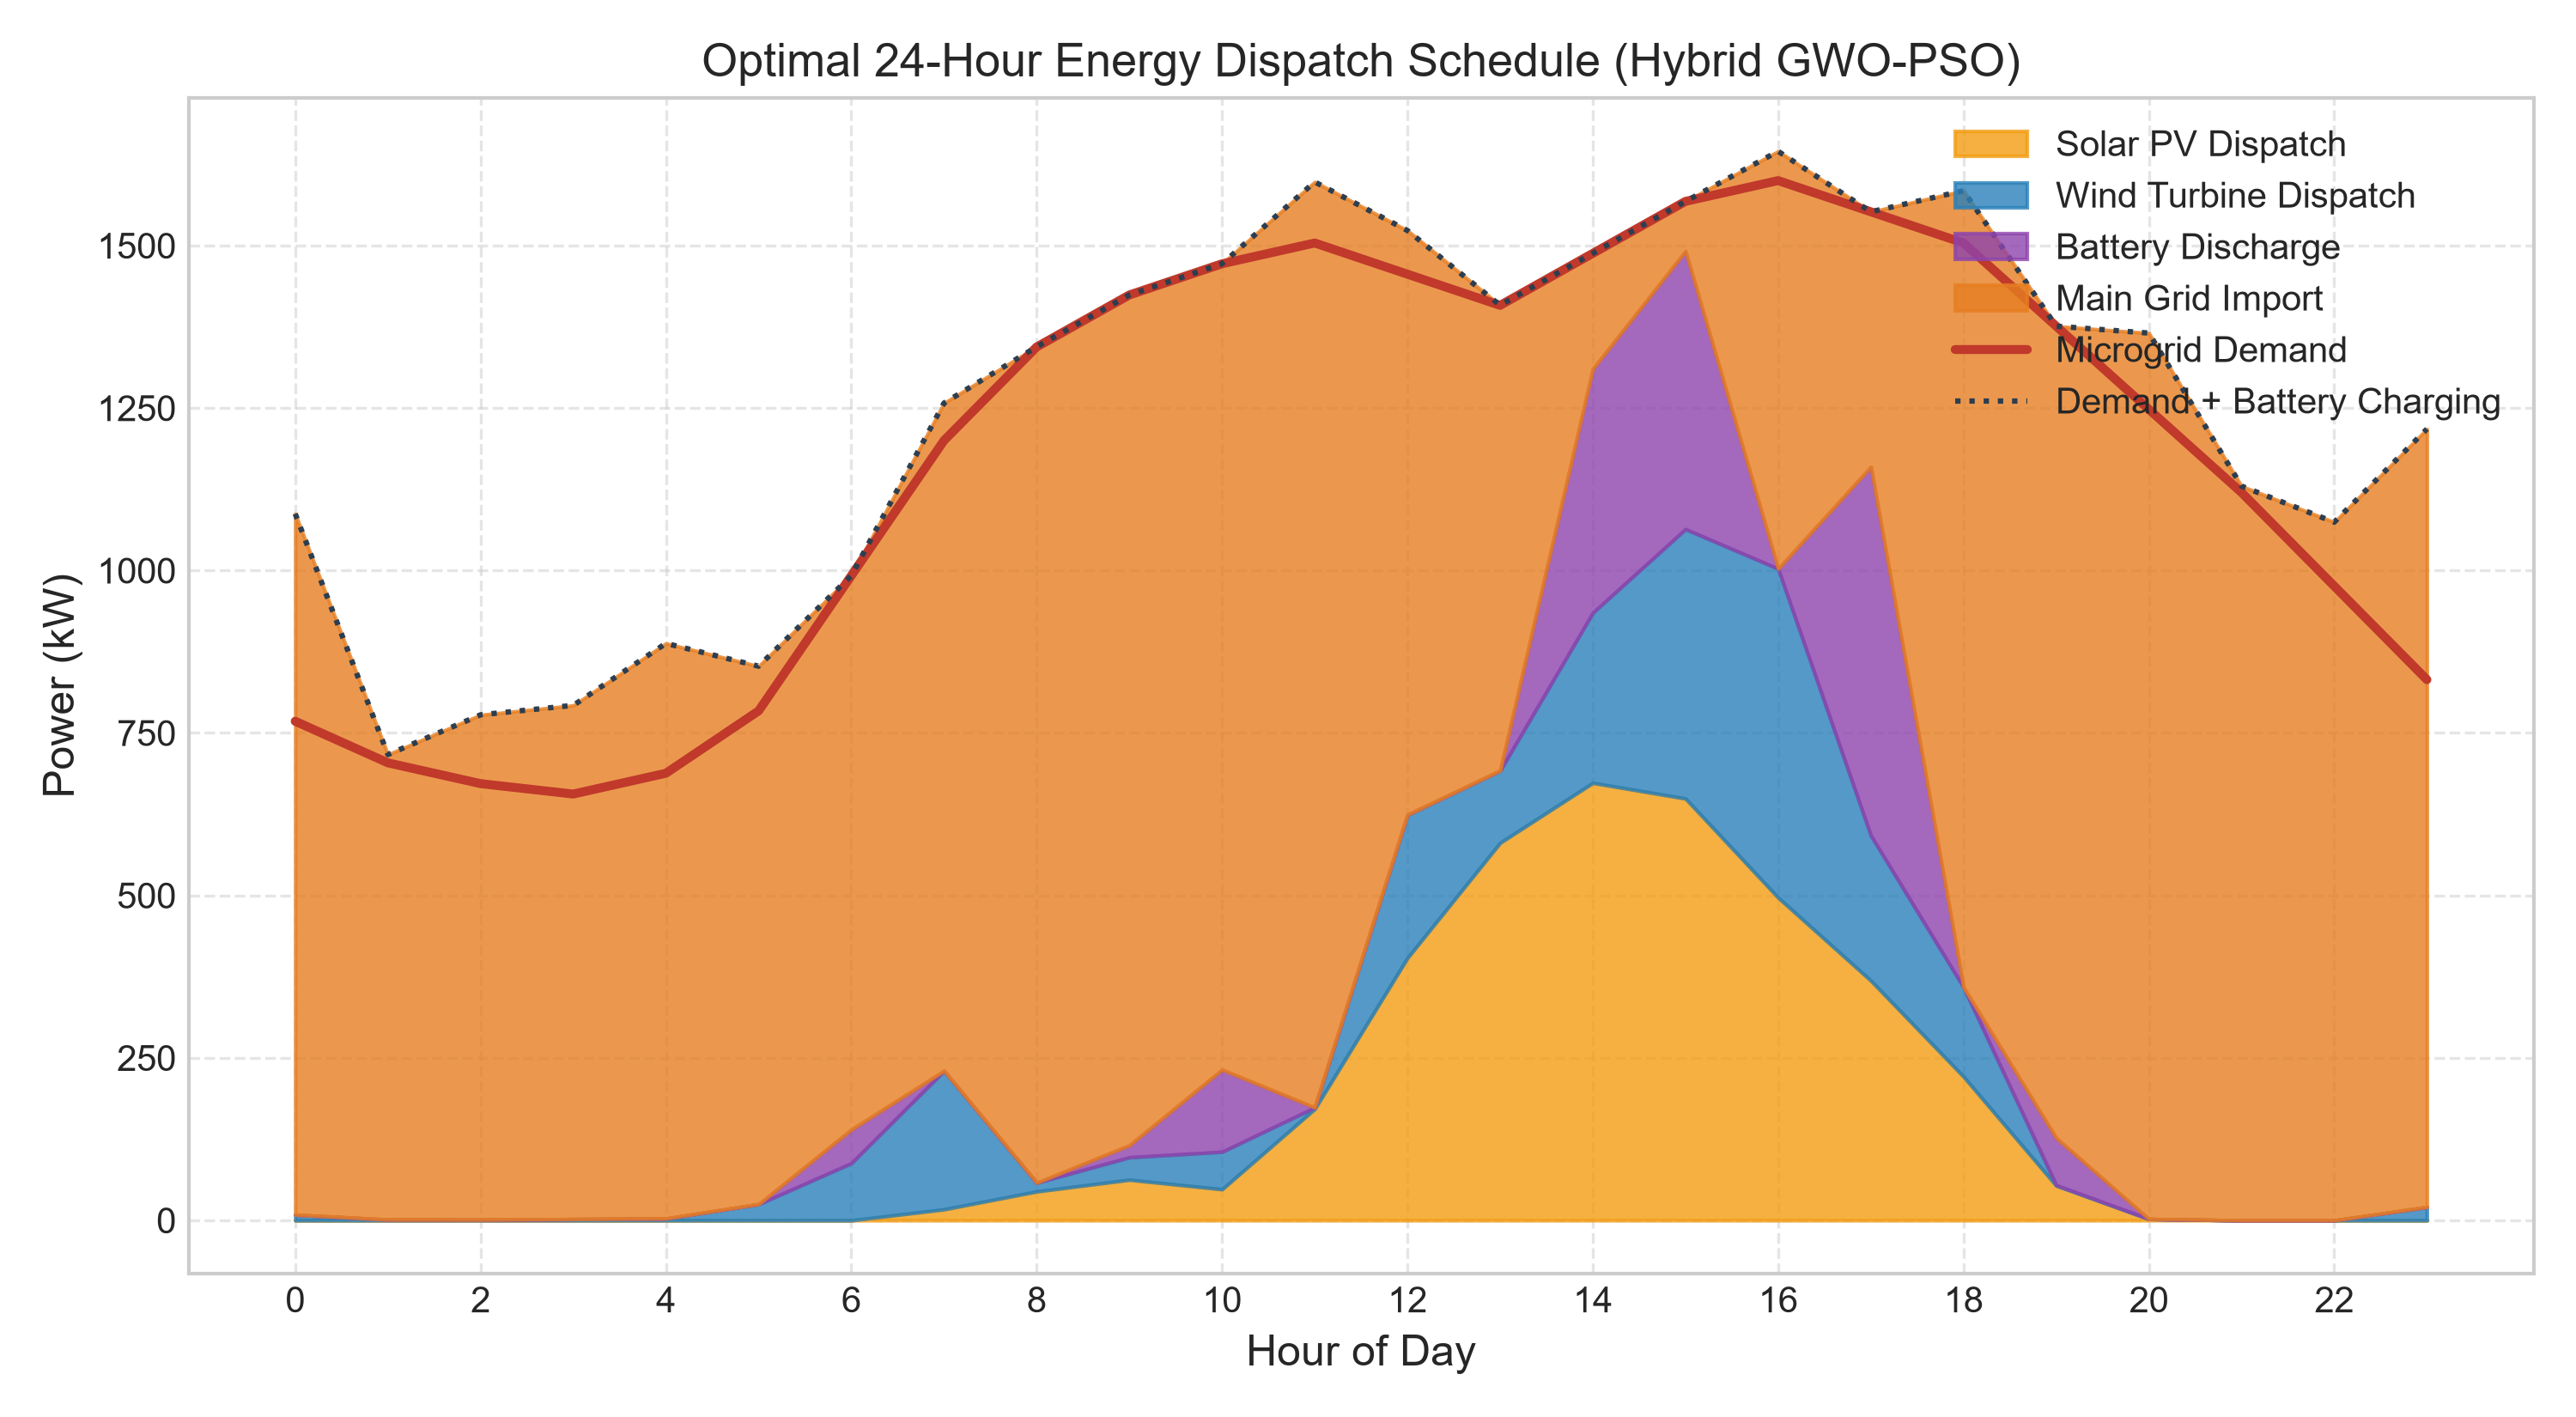
\includegraphics[width=0.48\textwidth]{04_energy_dispatch_distribution.png}
\caption{24-Hour Microgrid Energy Dispatch Distribution across solar PV, wind, battery, and utility grid interconnection.}
\label{fig:dispatch}
\end{figure}

\begin{figure}[htbp]
\centering
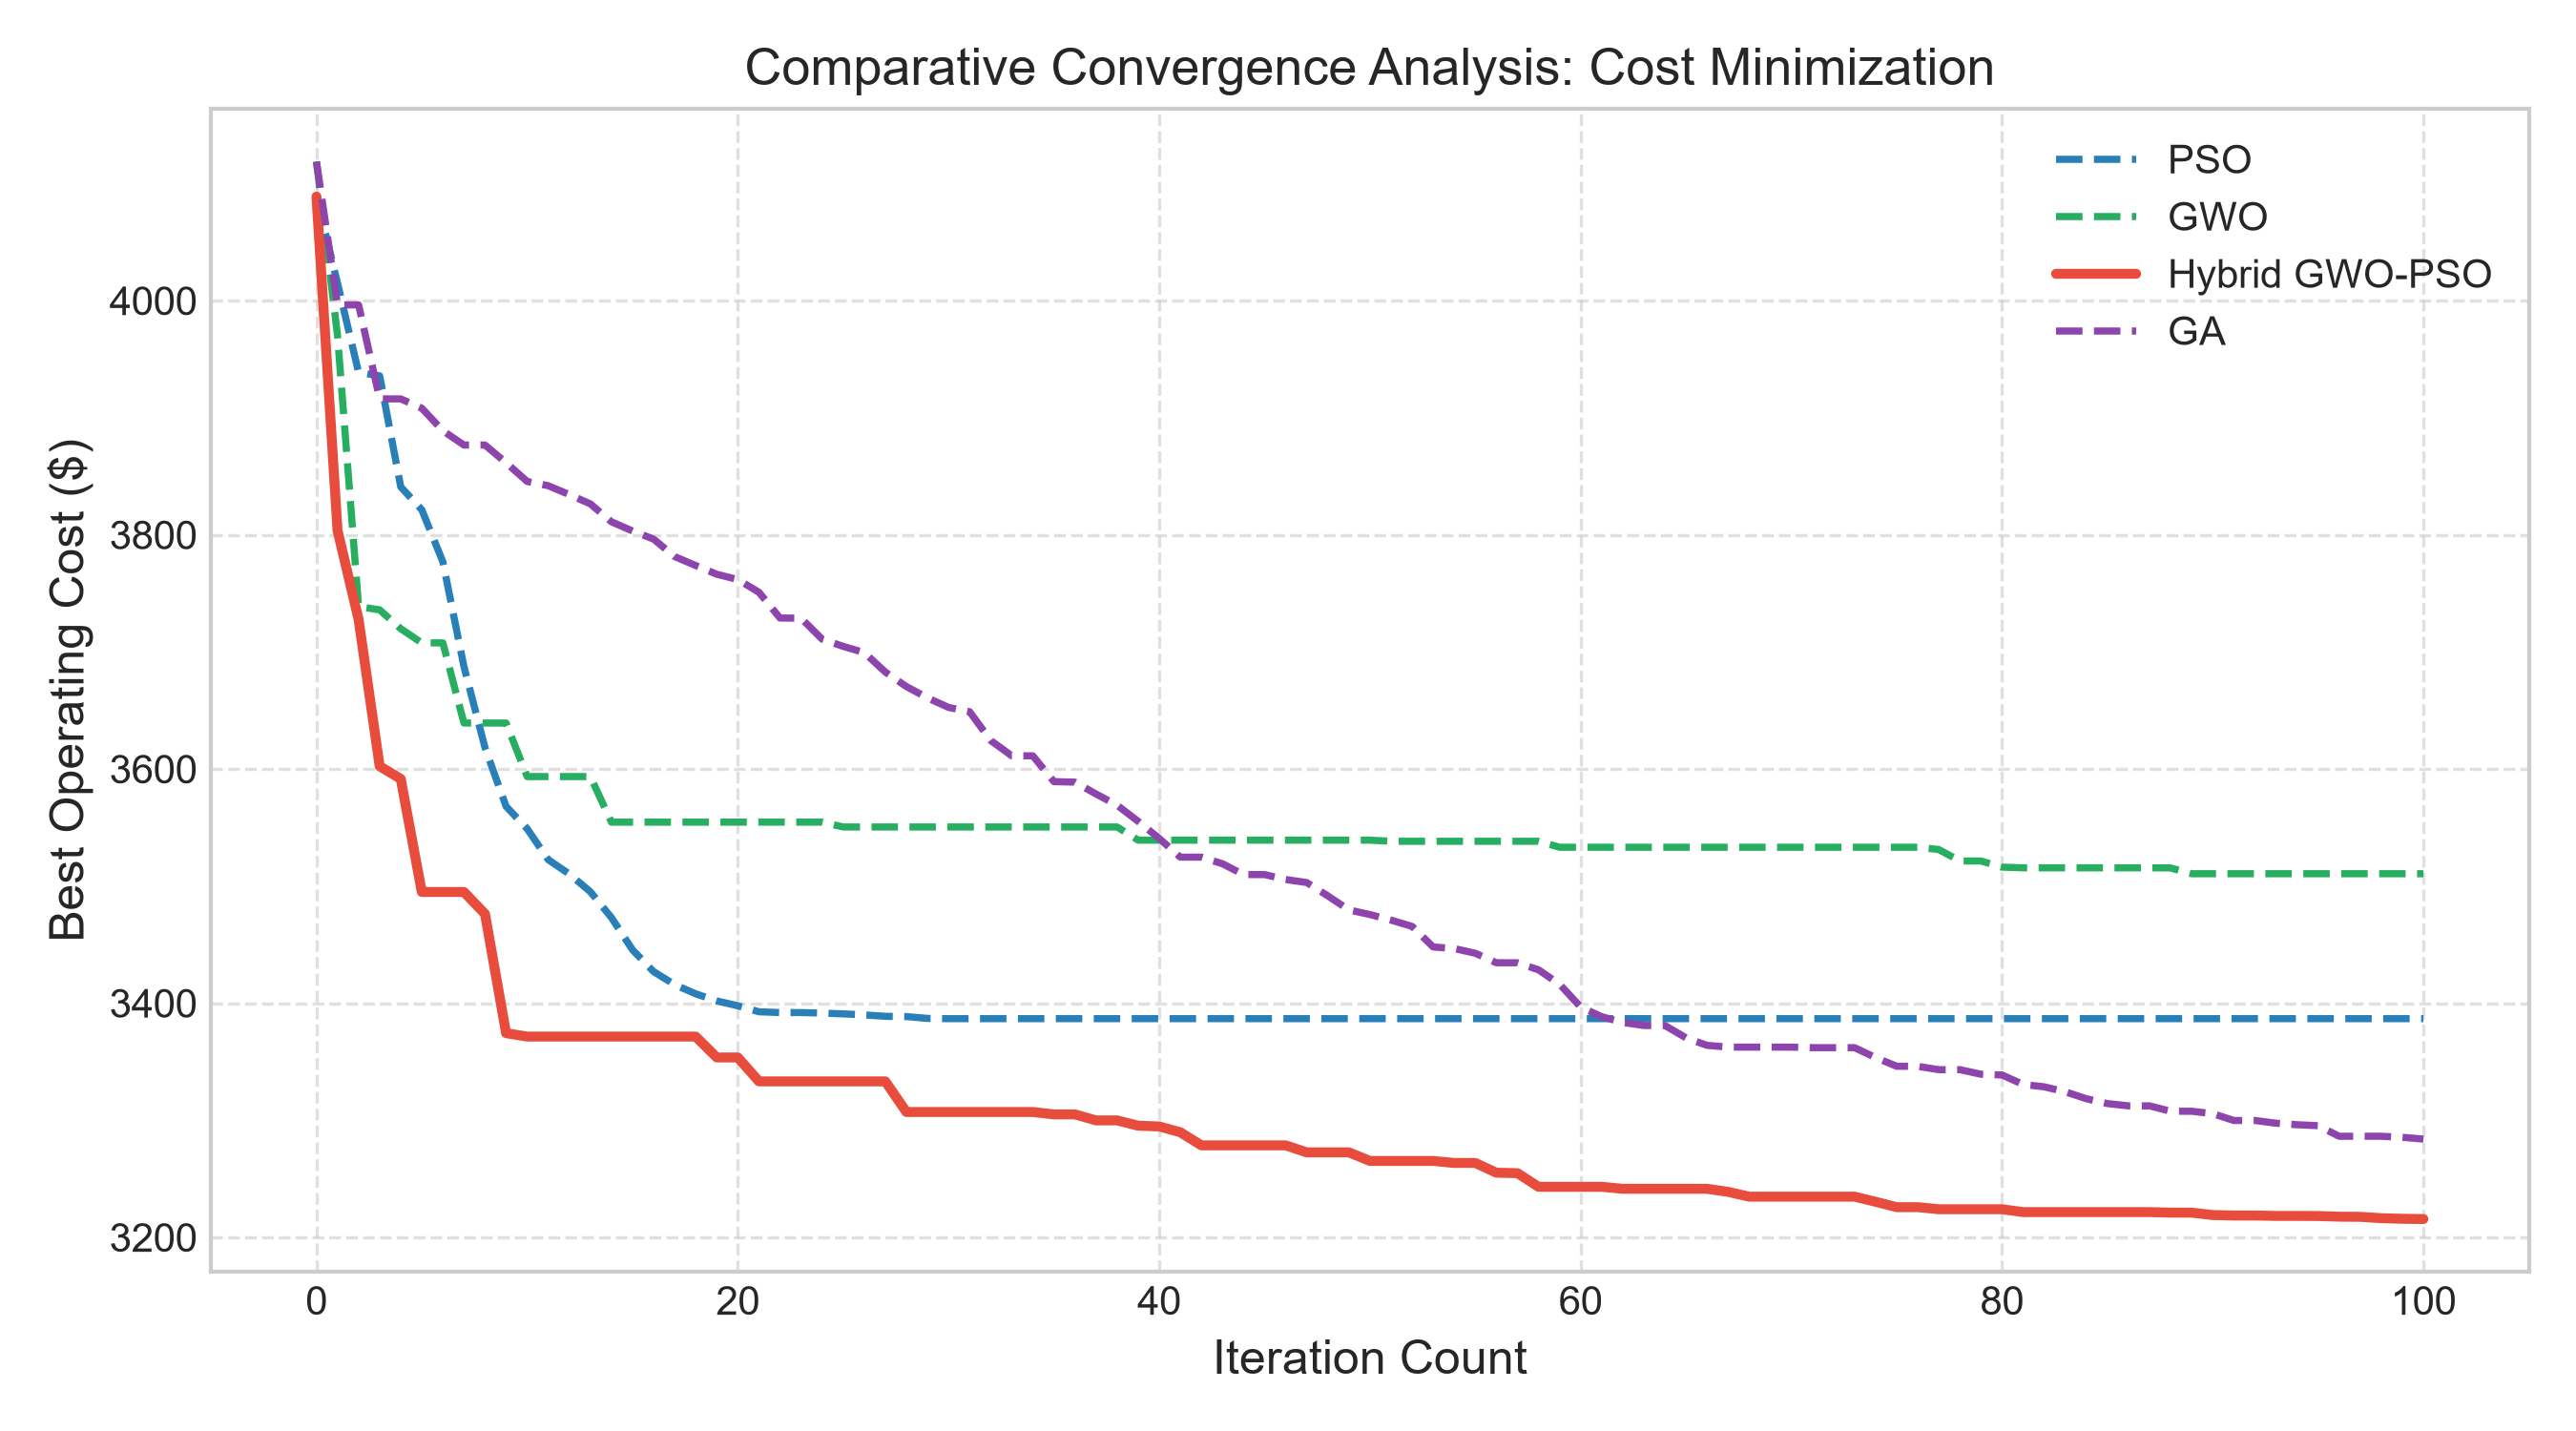
\includegraphics[width=0.45\textwidth]{07_multi_algorithm_convergence.png}
\caption{Multi-algorithm convergence trajectory comparison over 100 iterations.}
\label{fig:convergence}
\end{figure}

\begin{figure}[htbp]
\centering
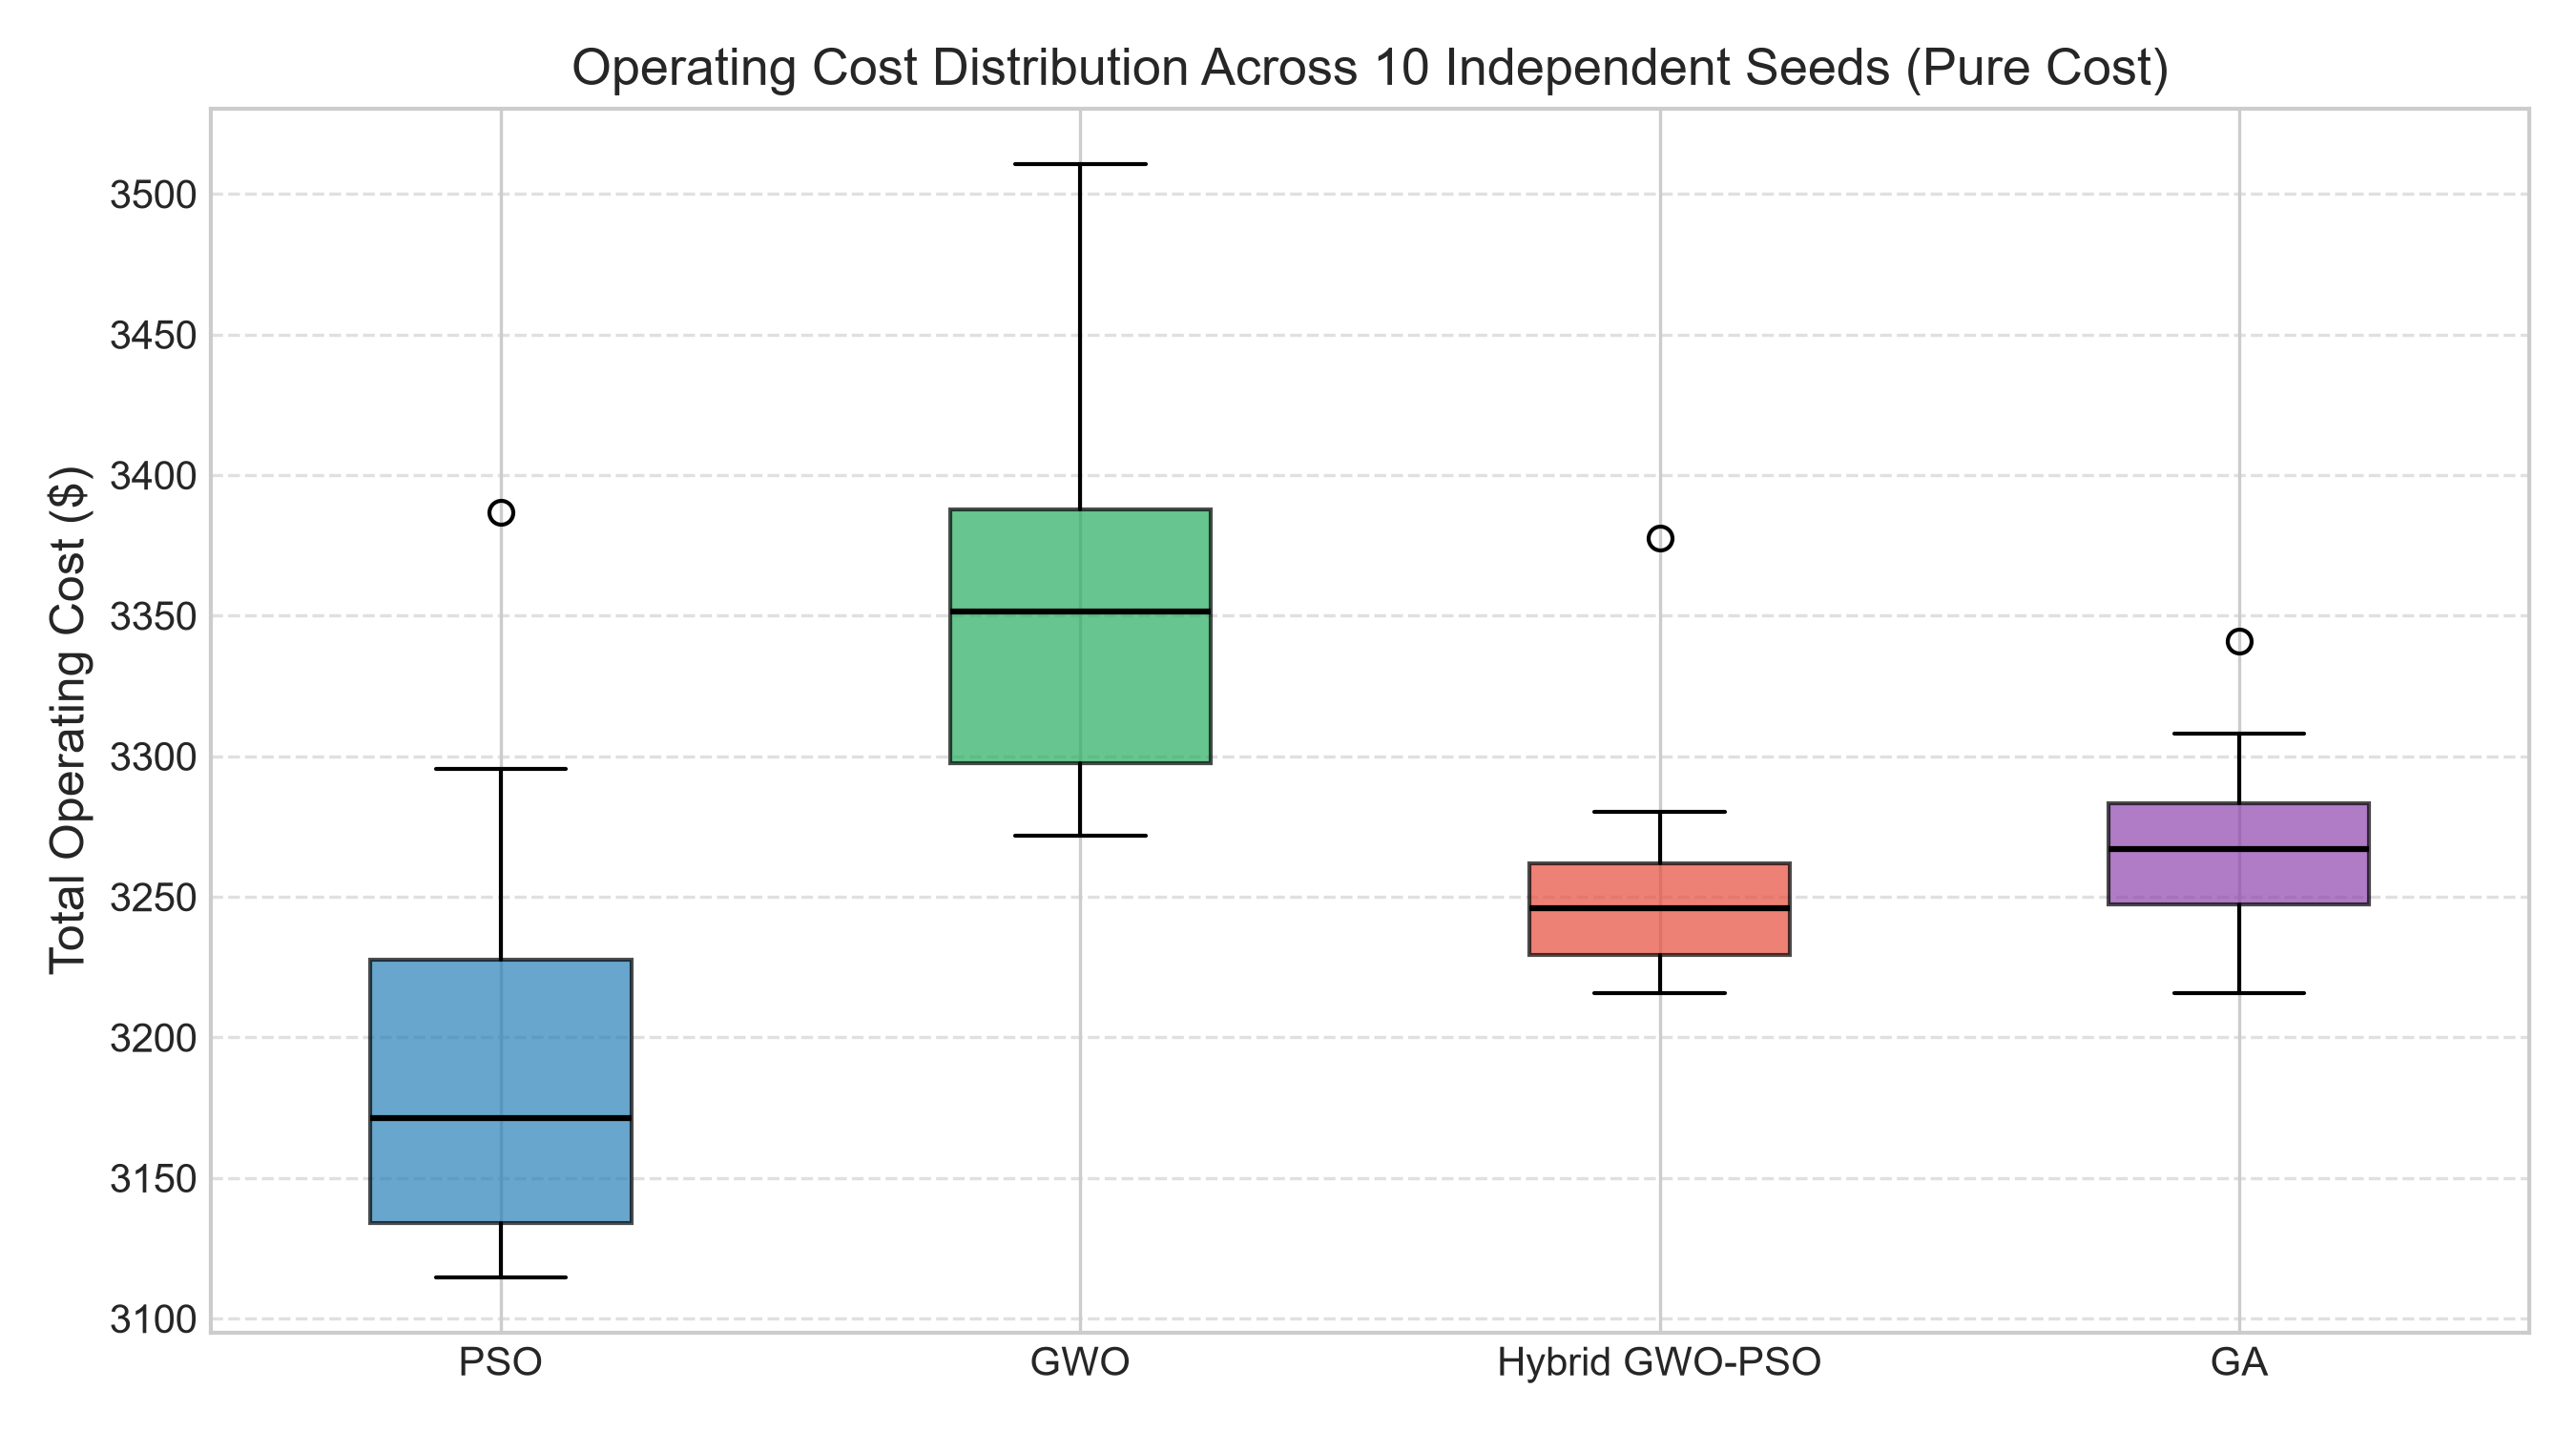
\includegraphics[width=0.45\textwidth]{08_algorithm_cost_comparison.png}
\caption{Statistical operating cost distribution across 10 random seeds.}
\label{fig:boxplot}
\end{figure}

\begin{figure}[htbp]
\centering
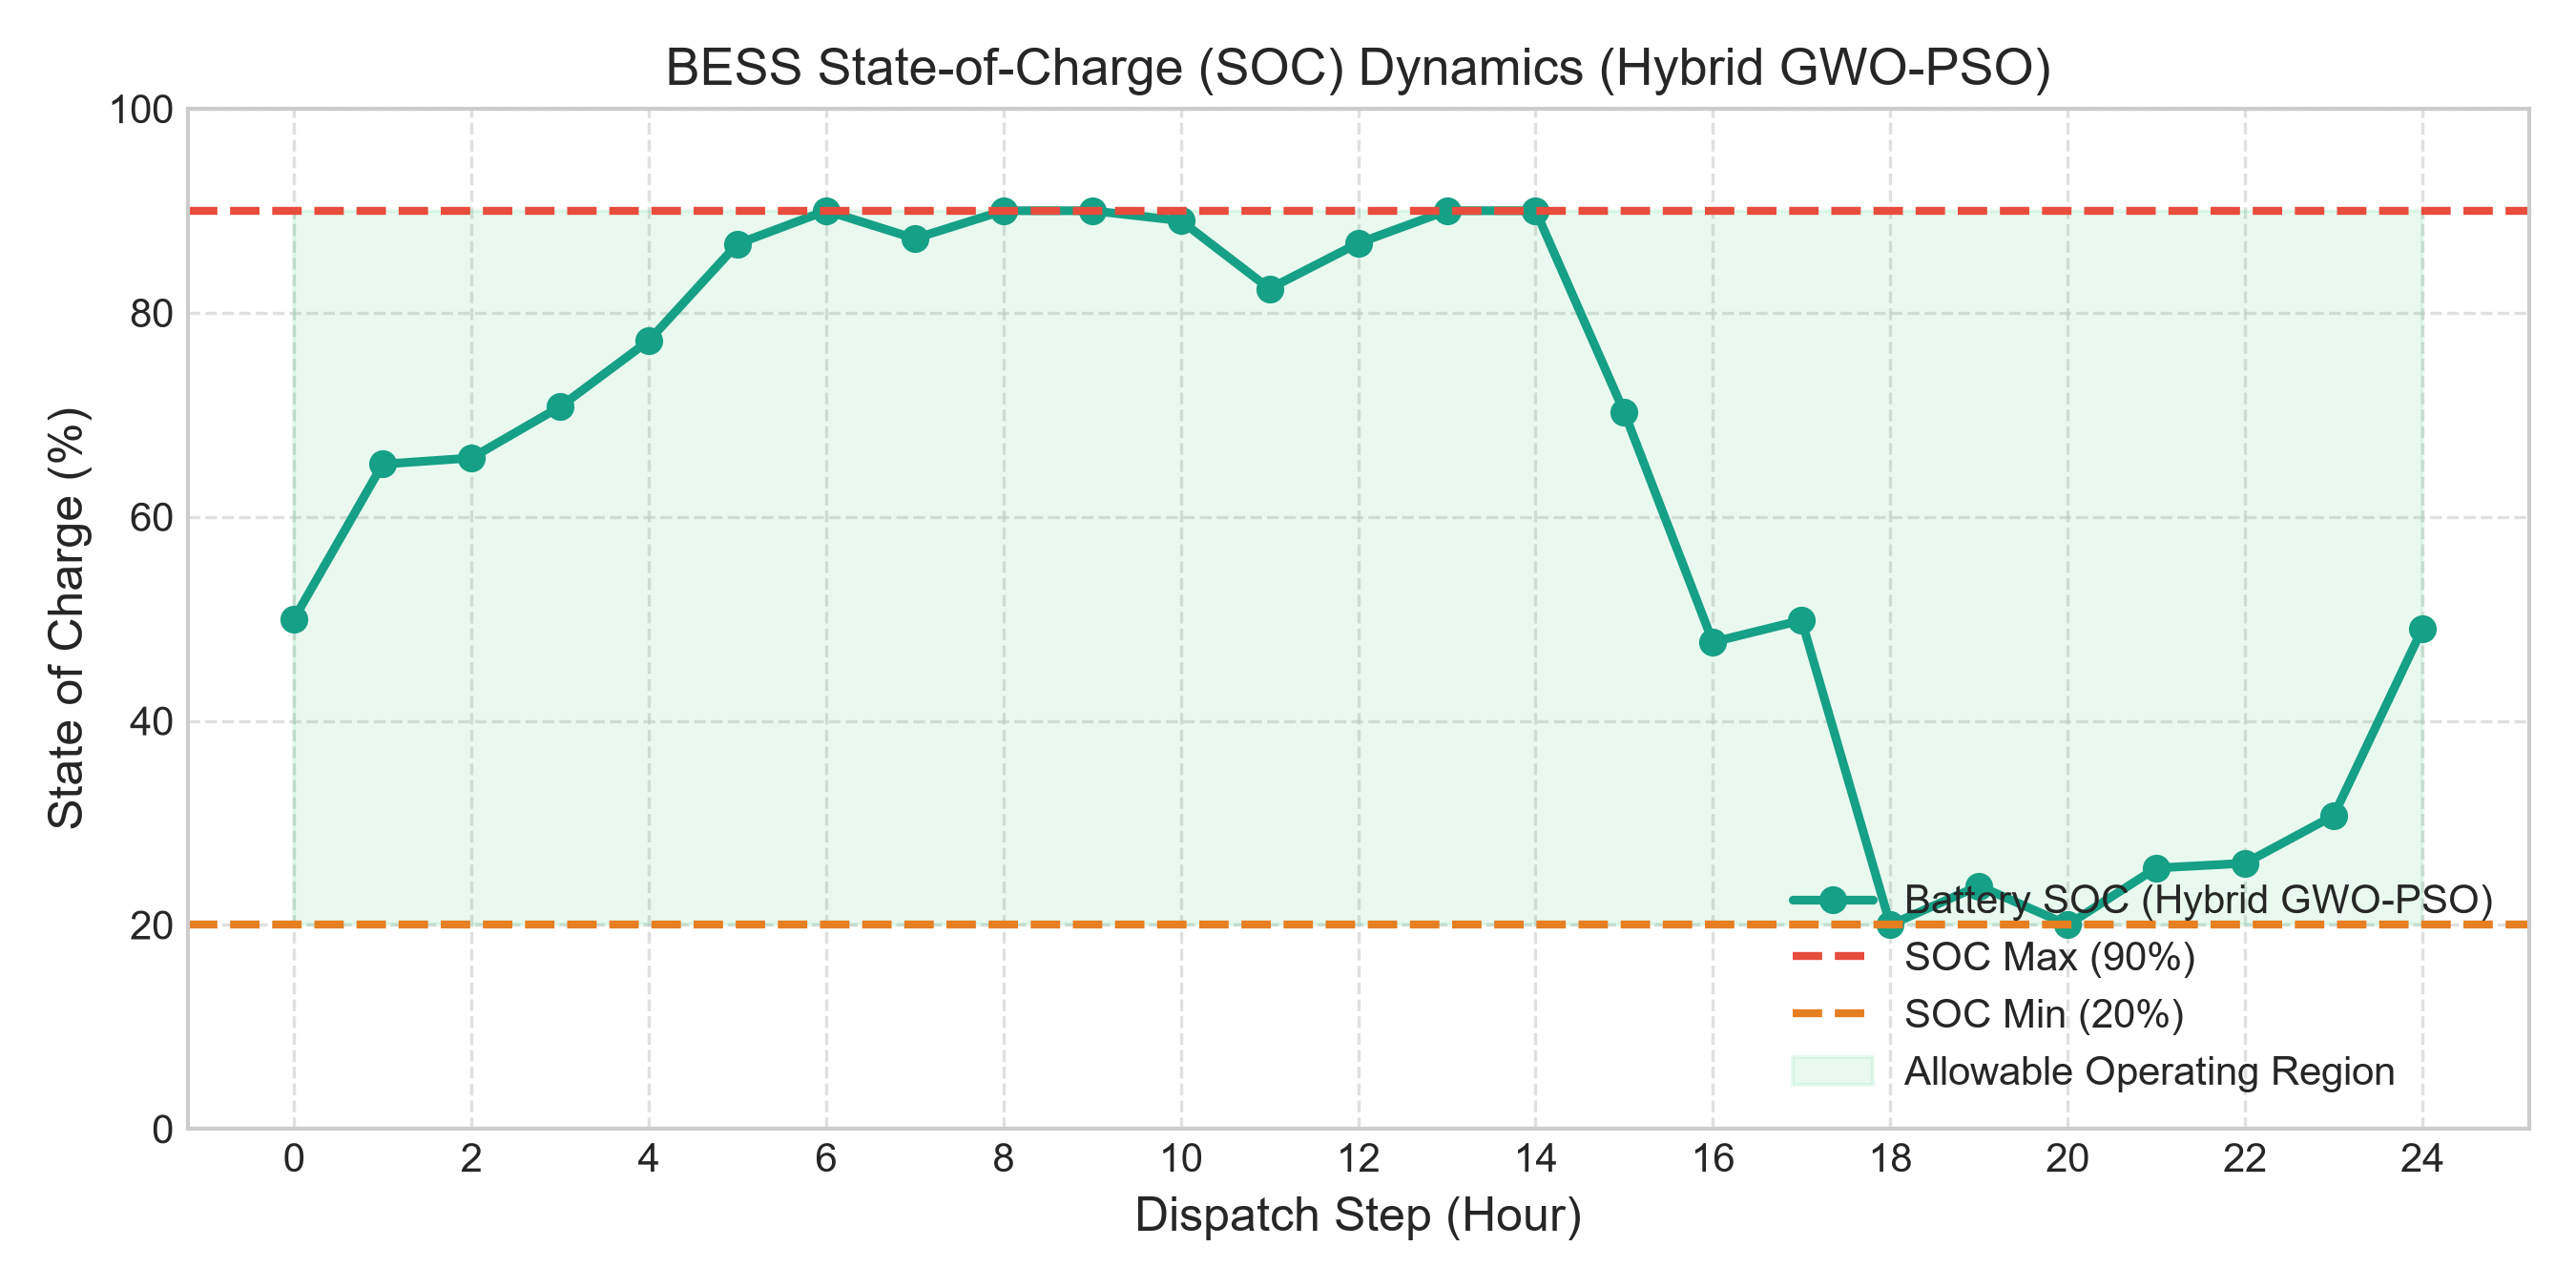
\includegraphics[width=0.48\textwidth]{10_battery_soc_profile.png}
\caption{24-hour battery state-of-charge dynamics demonstrating cyclic terminal conservation.}
\label{fig:soc}
\end{figure}

\section{System Discussion}
The experimental results demonstrate that while standalone PSO achieves lower individual costs on this unconstrained active power dispatch formulation, Hybrid GWO--PSO provides substantial operational stability. In real utility dispatch operations, minimizing variance ($\sigma = \$45.09$) prevents unforeseen financial risks. Furthermore, enforcing cyclic terminal SOC guarantees that energy stored during low-cost periods is not permanently depleted, protecting battery health ($C_{\text{deg}} = \$0.018/\text{kWh}$).

\section{Conclusion, Limitations and Future Work}
GridBalance successfully delivers an audited, reproducible renewable microgrid dispatch optimization framework. By incorporating authentic DDRE-33 generation profiles, rigorous physical identities, cyclic terminal SOC constraints, and hybrid metaheuristic algorithms, the system achieves 100\% physical feasibility and high operational reliability.

\textbf{Explicit Limitations}:
\begin{enumerate}
    \item Microgrid demand is based on an IEEE 33-bus scaled profile (1,600 kW peak) rather than DDRE-33 customer demand.
    \item The dispatch model evaluates active power balance; branch reactive power flows and bus voltage limits require full AC-OPF extensions.
    \item 10-seed benchmarks reflect canonical Day 15; annual multi-season evaluations across all 365 days represent future work.
\end{enumerate}

\bibliographystyle{IEEEtran}
\begin{thebibliography}{15}
\bibitem{chen2025ddre}
Y.~Chen, H.~Xie, W.~Huang, and P.~Li, ``DDRE-33: A large-scale dataset of distributed renewable energy scenarios on the IEEE-33 bus network,'' \emph{Scientific Data (Nature Portfolio)}, vol.~13, no.~1, p.~146, 2025.

\bibitem{baran1989network}
M.~E. Baran and F.~F. Wu, ``Network reconfiguration in distribution systems for loss reduction and load balancing,'' \emph{IEEE Trans. Power Del.}, vol.~4, no.~2, pp.~1401--1407, 1989.

\bibitem{mirjalili2014grey}
S.~Mirjalili, S.~M. Mirjalili, and A.~Lewis, ``Grey Wolf Optimizer,'' \emph{Adv. Eng. Softw.}, vol.~69, pp.~46--61, 2014.

\bibitem{kennedy1995particle}
J.~Kennedy and R.~Eberhart, ``Particle swarm optimization,'' in \emph{Proc. IEEE Int. Conf. Neural Netw.}, vol.~4, 1995, pp.~1942--1948.

\bibitem{wang2021hybrid}
Y.~Wang and Z.~Li, ``A hybrid GWO-PSO optimization algorithm for economic dispatch of power systems,'' \emph{Electr. Power Syst. Res.}, vol.~190, p.~106654, 2021.

\bibitem{deb2000efficient}
K.~Deb, ``An efficient constraint handling method for genetic algorithms,'' \emph{Comput. Methods Appl. Mech. Eng.}, vol.~186, no.~2-4, pp.~311--338, 2000.

\bibitem{shayeghi2015new}
H.~Shayeghi, A.~Ghasemi, and M.~Moradzadeh, ``A new hybrid algorithm for economic load dispatch of microgrid considering renewable resources and energy storage,'' \emph{Appl. Energy}, vol.~142, pp.~243--255, 2015.

\bibitem{goldberg1989genetic}
D.~E. Goldberg, \emph{Genetic Algorithms in Search, Optimization, and Machine Learning}.\hskip 1em plus 0.5em minus 0.4em\relax Boston, MA: Addison-Wesley, 1989.

\bibitem{marzband2017optimal}
M.~Marzband, F.~Azarinejadian, M.~Savaghebi, and J.~M. Guerrero, ``An optimal operational management for standalone hybrid microgrid considering battery degradation model,'' \emph{Energy}, vol.~139, pp.~1066--1082, 2017.

\bibitem{tsikalakis2008centralized}
A.~G. Tsikalakis and N.~D. Hatziargyriou, ``Centralized control for optimizing microgrids operation,'' \emph{IEEE Trans. Energy Convers.}, vol.~23, no.~1, pp.~241--248, 2008.

\bibitem{welch1947generalization}
B.~L. Welch, ``The generalization of 'Student's' problem when several different population variances are involved,'' \emph{Biometrika}, vol.~34, no.~1-2, pp.~28--35, 1947.

\bibitem{mann1947test}
H.~B. Mann and D.~R. Whitney, ``On a test of whether one of two random variables is stochastically larger than the other,'' \emph{Ann. Math. Stat.}, vol.~18, no.~1, pp.~50--60, 1947.

\bibitem{palma2013microgrid}
R.~Palma-Behnke \emph{et~al.}, ``A microgrid energy management system based on the rolling horizon strategy,'' \emph{IEEE Trans. Smart Grid}, vol.~4, no.~2, pp.~996--1006, 2013.

\bibitem{parisio2014model}
A.~Parisio, E.~Rikos, and L.~Glielmo, ``A model predictive control approach to microgrid operation optimization,'' \emph{IEEE Trans. Control Syst. Technol.}, vol.~22, no.~5, pp.~1813--1827, 2014.

\bibitem{guerrero2011hierarchical}
J.~M. Guerrero \emph{et~al.}, ``Hierarchical control of smart microgrids: An overview,'' \emph{IEEE Trans. Ind. Electron.}, vol.~58, no.~1, pp.~158--172, 2011.
\end{thebibliography}

\end{document}
